\documentclass[12pt]{article}
\usepackage[margin = 2.4cm]{geometry} % For margins of 3cm
\usepackage{gensymb} % For some symbols
\usepackage{amsmath} % All three for maths symbols
\usepackage[export]{adjustbox} % For figure frames
\setlength{\parskip}{6pt} % To make nice looking paragraph spacing
\usepackage[export]{adjustbox} % For figure frames
\usepackage{natbib} % bibliographies
\usepackage{natbib}
\usepackage[section]{placeins}
%\usepackage[backend=bibtex,firstinits=true]{biblatex}
\usepackage{setspace} % Allows double spacing
\usepackage{pdfpages} % Allows including PDFs
 \usepackage{lscape}
 \usepackage{courier}
\usepackage{lscape} % To allow some pages to be in landscape
\usepackage{float, subfloat} % For H flag and subfloats
\usepackage{caption, subcaption} % for ABCD Subcaptions
\usepackage[framemethod=tikz]{mdframed} % Allows coloured boxes
\hyphenpenalty 100000
\usepackage{titling}
\newcommand{\subtitle}[1]{%
	\posttitle{%
		\par
	\end{center}
	\begin{center}\large#1\end{center}
	\vskip0.5em}
}

\pagebreak
\doublespacing % Makes all lines (not figure legends) double spaced



\title{Effect of DHODH Deficiency on p53 Expression and Osteoblast Differentiaion in Miller's Syndrome Mouse Model}
\subtitle{\textbf{Preliminary RHEP}}
\author{ \textbf{Urwah Nawaz} \\ \textbf{a1654797}}

\date{}


\begin{document}
	\maketitle
	\pagenumbering{gobble}
	\pagenumbering{arabic}
	\paragraph{Declaration:}
	~\\This work does not contain any material written by another person, except where due reference is given in the text, and the work has not been presented previously as a component of any other academic course.	
	\paragraph{Word Count: 2494}
	~\\ Word count includes titles and figure legends, but excludes in-text references, appendices and acknowledgements 
\pagebreak
\paragraph{Hypothesis}
~\\ Dhodh deficiency causes an increase in p53 levels which subsequently repress Osterix/Sp7 during embryonic development in Miller's syndrome mouse model. 

	\section{Background}
	The developments of the face and limbs are intricate processes tightly regulated by signalling pathways and transcription factors (TFs) \citep{karsenty2009genetic}. Misregulation of these processes in the developing embryo leads to skeletal anomalies affecting approximately 1 in 3000 births \citep{stoll1989birth}. Miller's syndrome (MS) (OMIM:263750) is a rare autosomal recessive congenital disorder characterised by craniofacial and postaxial limb abnormalities \citep{miller1979postaxial}. These abnormalities include severe micrognathia, cleft lip and/or palate, and hypoplasia or aplasia of the posterior elements of the limbs.  The mechanisms underlying the aetiology of MS are incompletely understood. 
	
	 \subsection{Cause of Miller's syndrome}
	MS is caused by compound heterozygous missense mutations in the protein coding regions of the \textit{DHODH} gene \citep{ng2010exome}.  A total of 14 different mutations in \textit{DHODH} have been reported \citep{ng2010exome, doi:10.1093/hmg/dds218}. Each patient tends to carry a different combination of mutations, which dictates the severity of the MS phenotype. 
	
	\textit{DHODH} gene contains nine exons that encode a 43-kDa protein dehydroorotate dehydrogenase (DHODH). DHODH is a key enzyme in the \textit{de novo} pyrimidine synthesis and localises in the inner mitochondrial membrane. DHODH catalyses the oxidation of dehydroorate to orotate, linking it to the  mitochondrial respiratory chain (MRC) by using ubiquinone as a substrate \citep{fang2013dihydro}. \textit{In vivo } and \textit{in vitro} assays revealed an overall reduced enzymatic DHODH activity from 11 MS associated alleles \citep{doi:10.1093/hmg/dds218}. Three disease-associated missense mutations were further evaluated, revealing reduced protein stability (G202A and R346W) or impairment in the substrate-induced enzymatic activity (R135C) \citep{fang2012protein}. These mutants retained their normal mitochondrial localisation. This implies that affected individuals have a deficiency of \textit{de novo} pyrimidine synthesis. No individual has been identified with both alleles showing severe loss-of-function (LOF) \citep{doi:10.1093/hmg/dds218}. Consistently, an upper and lower threshold for DHODH activity has been established, where greater than 50\% activity results in a normal phenotype, but insufficient activity leads to embryonic lethality \citep{doi:10.1093/hmg/dds218}. The mechanisms by which DHODH deficiency causes the MS phenotype are not clear. 


\subsection{DHODH deficiency and  p53 activation }
	Selective inhibition of pyrimidine biosynthesis is used as a therapeutic approach to treat various cancers and autoimmune disorders \citep{ren2017leflunomide, liu2017inactivation, leban2011human}. Leflunomide, converted to the active metabolite, Teriflunomide, reduces \textit{de novo} pyrimidine biosynthesis by selectively inhibiting DHODH (Figure \ref{fig:inhibition}). 
	 
	 \begin{figure}[!htp]
	 	\centering
	 	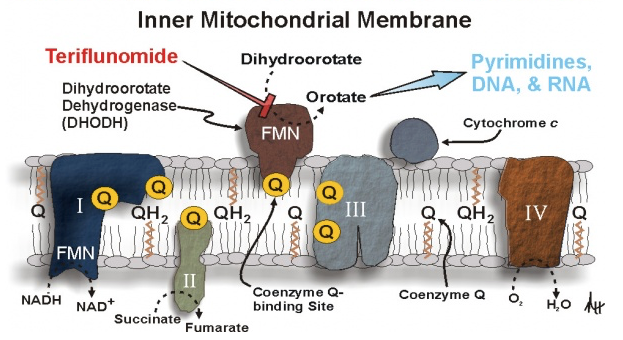
\includegraphics[width=0.55\linewidth]{Pictures/inhibition}
	 	\caption{Teriflunomide inhibits DHODH thereby causing an impairment in the pyrimidine nucleotide pool, and defective MRC complex III. Reproduced from \cite{velez2013mitochondrial}}
	 	\label{fig:inhibition}
	 \end{figure}
	 
	Cancer cell-lines treated with leflunomide show that DHODH inhibition leads to a depletion in the pyrimidine nucleotide pool, and generation of reactive oxygen species (ROS), via mitochondrial dysfunction. These effects have contributed to an increase in p53 levels, which inhibit cell proliferation, induce cell-cycle arrest, and cause p53 dependent apoptosis in human cancer-cell lines  \citep{linke1996reversible, khutornenko2010pyrimidine, hail2012evidence, fairus2017dihydroorotate}. 
	
	A common feature among several craniofacial abnormalities is p53 activation however the mechanisms involved are not completely elucidated \citep{jones2008prevention, barlow2010p53, boultwood2012haploinsufficiency, sakai2016prevention}. Mutations in the \textit{Tcof1} gene in Treacher Collins Syndrome (TCS), lead to an increase p53 levels in the neuroepithelium of the TCS mouse model. Knock-out (KO) and pharmacological inhibition of p53 ameliorates the craniofacial phenotype in the TCS mouse model \citep{jones2008prevention, sakai2016prevention}. Similarly, p53 stabilization in cranial neural crest cells (CNCC) leads to craniofacial defects in mouse and chick embryos, indicating that p53 coordinates CNCC growth by affecting cell cycle gene expression and proliferation at discrete developmental stages \citep{Rinon1827}. It is possible that DHODH deficiency causes an up-regulation in p53 that lead to the defects observed in MS.
	
	While evidence supports that DHODH deficiency leads to an increase of p53, some studies have shown conflicting results. Previously, siRNA-mediated DHODH depletion in HeLa cells showed no difference in p53 levels \citep{fang2013dihydro}. Additionally, treatment with leflunomide in null-p53 mutant zebrafish led to a decrease in migrating neural crest cells \citep{white2011dhodh},  suggesting that DHODH may function in a p53 independent manner. However, these results could be attributed to tissue-specific variation and thus the involvement of p53 in MS warrants further investigation.
	
	\subsection{Craniofacial and Limb Development}
	MS diagnose is associated with defective craniofacial and limb development. Internal malformations are uncommon in MS patients \citep{doi:10.1093/hmg/dds218}, implying that the developmental pathways affected in MS disrupt cartilage and bone development. Consistently, the mouse orthologue, \textit{Dhodh } showed spatio-temporal expression during E10.5 (Embryonic day post coitum) in craniofacial region, hindlimbs and forelimbs \citep{doi:10.1093/hmg/dds218}. 
	
	 The differentiation of osteoblasts from the mesenchymal precursors is controlled by a hierarchy of TFs including Runx2 and Osterix (or SP7) \citep{karsenty2009genetic}. Conditional inactivation of Osx/SP7 in CNCC has resulted in defective craniofacial bone development in mice  \citep{baek2013osterix}. Additionally, a human patient with a homozygous mutation in Osx/SP7 displayed craniofacial and limb bone deformities \citep{lapunzina2010identification} inclduing midface hypoplasia, micrognathia,  and asymmetry of the limbs. These phenotypes overlap with MS phenotype.
	 	
	p53 exerts a repressive effect on osteoblast differentiation and bone development \citep{ohyama1997p53, wang2006p53}. In osteosarcoma development, LOF of p53 causes abnormal osteogenesis, and up-regulation of Runx2 and Osx/SP7 \citep{berman2008metastatic}. Similarly, p53 is able to directly repress Osx causing a decrease in osteoblast differentiation \citep{p53sp7}.  Thus, the p53-mediated inhibition of Osx might have implications in bone formation under pathological conditions during embryonic development.
	
	In MC3T3-E1 cells, depletion of DHODH activity decreases osteogenic gene expression. Expression and protein levels of p53 increased in this study, although the relationship between p53 and osteoblast differentiation was not explored. MC3T3-E1 cells contain Osx/SP7  \citep{tian2012osterix}. \textit{Osx} mRNA levels in mice show significant up-regulation between E11.5 and E13.5, subsequent to the increased \textit{Dhodh} expression at E10.5 \citep{ gao2004molecular,  kaback2008osterix, doi:10.1093/hmg/dds218}. It is possible that one of the mechanisms by which DHODH deficiency (as a result of the mutations) leads to the MS phenotype is  by increasing p53 levels which subsequently represses Osx/SP7 (Figure \ref{fig:proposedmechanism}). 

\pagebreak
\section{Experimental Overview}
\subsection{Proposed model}

	
\begin{figure}[!htp]
	\centering
	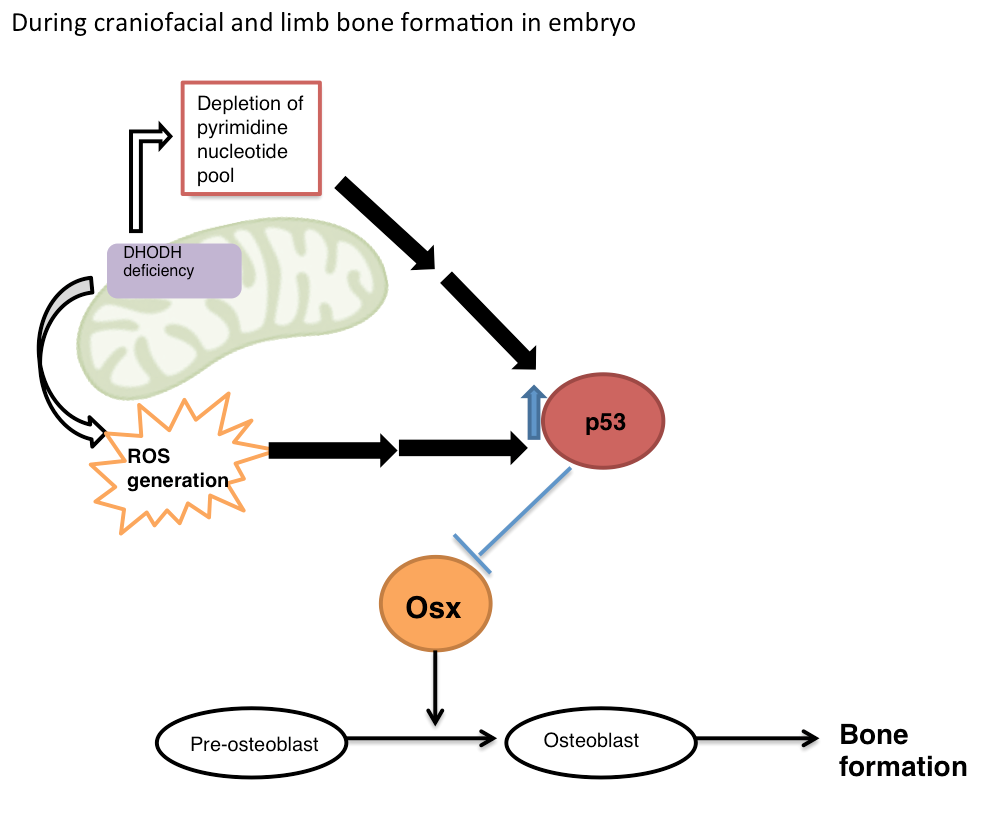
\includegraphics[width=0.7\linewidth]{Pictures/proposed_mechanism}
	\caption{Illustration of the proposed model. DHODH mutations cause Dhodh deficiency leading to mitochondrial dysnfuntion and depletion of pyrimidine nucleotide pool. As a result, p53 levels are increased and subsequently repress Osterix/SP7 during embryonic development}
	\label{fig:proposedmechanism}
\end{figure}

\subsection{Experimental Aims}

\paragraph{Aim 1:} To generate a mouse model system for Miller's Syndrome using CRISPR-Cas9 
\paragraph{Aim 2:} To determine if p53 levels are increased during craniofacial and limb development due to Dhodh deficiency by using mRNA and protein quantification techniques
\paragraph{Aim 3:} To determine if Osx/SP7 is being repressed due to increased p53 levels via Dhodh deficiency using quantitative Real Time-PCR and Proximity Ligation Assay

\subsection{Experimental Plan}
\begin{figure}[!htp]
	\centering
	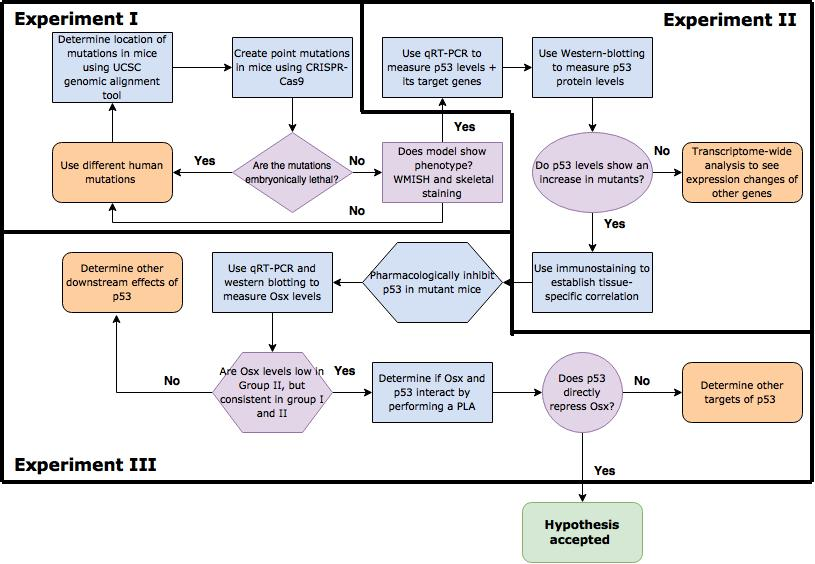
\includegraphics[width=0.95\linewidth]{Pictures/flowchart9}
	\caption{Flowchart and Summary of Experimental plan. Blue: Experiments; Purpler: Experimental questions; and Orange: Alternative experiments if desired results not obtained.}
	\label{fig:flowchat}
\end{figure}

\subsection{Controls for the experiment}


\begin{table}[!htp]
	\centering
	\caption{Mice and controls for this study}
	\label{controls}
	\begin{tabular}{|l|l|l|l|}
		\hline
		Mice                                                                            & Description                                                                       & Treatment                                                                                                   & Group \\ \hline
		Wildtype mouse (WT)                                                             & C57BL/6J mice embryos                                                                     & Control                                                                                                     & I     \\ \hline
		\textit{Dhodh} mutant mice                                                               & \begin{tabular}[c]{@{}l@{}}Mice embryos maintained \\ on C57BL/6J background\end{tabular} & \begin{tabular}[c]{@{}l@{}}Mice generated using \\ CRISPR/Cas9 as described \\ in Experiment 1\end{tabular} & II    \\ \hline
		\begin{tabular}[c]{@{}l@{}}\textit{Dhodh} mutant mice embryos\\  with p53 inhibitor\end{tabular} & \begin{tabular}[c]{@{}l@{}}Mice embryos maintained\\ on C57BL/6J background\end{tabular} & \begin{tabular}[c]{@{}l@{}}Mice treated with\\ pifithrin-$\alpha$ as described \\ in Experiment III\end{tabular}    & III   \\ \hline
	\end{tabular}
\end{table}

The embryos will be obtained by timed mating; the morning of the vaginal plug is considered to be E0.5.  Embryos will be collected as described by \cite{piliszek2011ex} at stages E9.5, E10,5, E11.5, E12.5, E13.5 and E14.5. Each experiment specifies at what stage the embryos are collected.  Three embryos from each group at each specific stage will be used for each experiment, unless otherwise specified. 


\section{Experiment I: Generation of mouse model for  Miller's syndrome}

\subsection{Proposed Experiments}
~\\ CRISPR-Cas9 will be used to introduce the human missense mutations p.R135C and p.E52G will be introduced into mice \textit{Dhodh}. USCS genomic tool will identify the corresponding mutations in mice \citep{kuhn2012ucsc}. Guide RNA (gRNAs) and single-stranded oligodeoxynucleotides (ssODNs) will be generated as previously detailed \citep{inui2014rapid} and examples are shown in Table \ref{mutation}. Potential off-target sites will be predicted using the algorithm determined by  \cite{Zheng} (2018). Examples of gRNAs and ssODNs are listed in Table \ref{my-table}.
\begin{table}[!htp]
	\footnotesize
	\centering
	\caption{Examples of gRNAs and ssODNs generated for base substitutions using CRISPR design tool by Zhang lab}
	\label{my-table}
	\begin{tabular}{lllll}
		Mutation                              & gRNAs                                              & ssODNs                                                                                                                                                                                       & \begin{tabular}[c]{@{}l@{}}Quality Score\\ of gRNA(\%)\end{tabular} & \begin{tabular}[c]{@{}l@{}}Off-target\\ score of gRNAs\end{tabular} \\ \hline
		\multicolumn{1}{|l|}{155A$>$G;p.E52G} & \multicolumn{1}{l|}{\texttt{5' TTGATCCAGAGTCGGCGCACCGG 3'}} & \multicolumn{1}{l|}{\begin{tabular}[c]{@{}l@{}}5' \texttt{TTTCTACGCCGA}\\ \texttt{GTACCTGATGCCG}\\ \texttt{GCTCTGCAGAGA}\\ \texttt{CTGCTTGATCCAG} \\ \texttt{\textbf{G} GTCGGCGCACC}\\ \texttt{GGCTAGCTGTTCG}\\ \texttt{AGTCATCTCCCTG}\\ \texttt{GGGCTCCTTC 3'}\end{tabular}} & \multicolumn{1}{l|}{97}                                         & \multicolumn{1}{l|}{0.3}                                            \\ \hline
		\multicolumn{1}{|l|}{403C$>$T;pR135C} & \multicolumn{1}{l|}{\texttt{5' CCGAGTATTCCGTCTCCCTGAGG 3'}} & \multicolumn{1}{l|}{\begin{tabular}[c]{@{}l@{}}\texttt{5'GTTGAGGTGGGAAG}\\ \texttt{TGTGACTCCCCAGCCT}\\ \texttt{CAGGAAGGAAACCCCA}\\ \texttt{GGCCCCGAGTATTC\textbf{T}GT}\\ \texttt{CTCCCTGAGGACCAAGC}\\ \texttt{TGTTATTAACAGG 3'}\end{tabular}}             & \multicolumn{1}{l|}{80}                                         & \multicolumn{1}{l|}{0.5}                                            \\ \hline
	\end{tabular}
\end{table}
Off-target hit scores are computed as 100\% minus a weighted sum of off-target hit-scores in the target genome taking into account the number of mismatches. 
The gRNA and ssODNs mixed in a hCas9 vector mRNA will be injected into mouse zygotes and transferred to  pseudo-pregnant females as described before \citep{inui2014rapid,  kato2013production, takada2013targeted}. Genomic DNA will be obtained and assessed for the presence of mutations in the \textit{Dhodh} gene. Mice harbouring mutant alleles will be bred to obtain $Dhodh^{E52G/R135C}$ pups. Point mutations will be confirmed by sequence analysis of genomic DNA extracted from individual embryos as described \citep{inui2014rapid}. For skeletal staining, the skeleton of E17.5 $Dhodh^{E52G/R135C}$ pups will be fixed in 99\% ethanol and stained for bone and cartilage as described \citep{baek2014skeletal}. In subsequent experiments, $Dhodh^{E52G/R135C}$ mice will be known as Group II. 
 \begin{figure}[!htp]
 	\centering
 	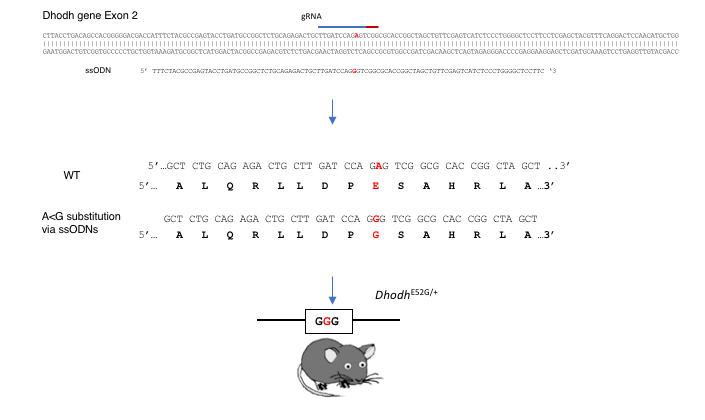
\includegraphics[width=1.00\linewidth]{Pictures/crispr}
 	\caption{Schematic illustration of showing the locations of a gRNA and ssODN used to generate the 155A$<$G base substitution, along with the exon 2 of \textit{Dhodh} gene, and expected genotype of the mouse. Blue bar indicates target of the gRNA with the red bar highlighting the PAM sequence. Red letters indicate the substitution target site in the \textit{Dhodh} locus and corresponding mismatched nucleotides in the ssODNs }
 	\label{fig:crispr}
 \end{figure}
 
Whole-mount \textit{in situ} hybridisation (WMISH) will be performed and fluorescence levels will be quantified as described before \citep{doi:10.1093/hmg/dds218} with probes specific for \textit{Dhodh} on Group I and Group II at E10.5. 


\subsection{Possible outcomes and interpretation}
Previously, leflunomide had been able to replicate the MS phenotype in zebrafish or mice \citep{white2011dhodh, fukushima2009inhibiting}. However, this approach was limited by the off-target effects of leflunomide, such as inhibiting tyrosine kinases.  \citep{fukushima2009inhibiting}. Therefore, by using CRISPR-Cas9, the mutations found in MS patients can be replicated in a mouse model, and provide a better understanding of DHODH deficiency in the developing embryo. 
The human point mutations p.E52G and p.R135C  selected because clinical details for the human carrier of these mutations had features most typical for the syndrome \citep{doi:10.1093/hmg/dds218}. Additionally, previous \textit{in vitro} analysis revealed that the residual activity for R135C is $>$50\%, whereas the activity for E52G is $<$10\% which gives a combination of a moderate LOF and a severe LOF allele, consistent with the threshold activity of DHODH \citep{doi:10.1093/hmg/dds218}. 

By using WMISH, expression levels of \textit{Dhodh} can be compared between WT and mutant. Lower \textit{Dhodh} expression should be expected in Group II.  Expected phenotype characteristics include: cleft palate, mandibular micrognathia in the craniofacial region, and anomaly of limb and digits, a short and/or tinted tail \citep{fukushima2009inhibiting}. These will be analysed using skeletal staining.  Normal Mendelian frequencies are expected: $Dhodh^{E52G/R135C}$, $Dhodh^{+/R135C}$ and  $Dhodh^{+/+}$ pups. As reported previously on \cite{mouse} (2018), global deletion of \textit{Dhodh} gene results in embryonic lethality, so mice homozygous for E52G will not be expected to survive.
 
It is possible that the point mutations will not result in the desired phenotype, or cause embryonic lethality. If this occurs, different human \textit{DHODH} mutations (Appendix A) should be generated in mice using the same strategy. 
 

\pagebreak

\section{Experiment II: Investigating p53 levels in Miller's syndrome mouse model}
\paragraph{Hypothesis:} p53 levels will show a spatiotemporal increase after E10.5 during mouse embryonic development.

\subsection{Proposed Experiments}
\paragraph{quantitative Real Time-PCR}
~\\\textit{Trp53}, \textit{Ccng1} , \textit{Trp53inp1}, \textit{Pmaip1}, \textit{Perp} and \textit{Wig1} will be analysed using qRT-PCR. Total RNA will be extracted from E9.5 through E12.5 Group I and II embryos using RNeasy Mini Protocol for Isolation of Total RNA from Animal Tissues (Qiagen), following the manufacturer's instructions. cDNA will be synthesised using a reverse transcription kit (Qiagen). \textit{Gadph} will serve as a house-keeping gene.  Quantitative analysis of each gene product will performed via RT-PCR using specific primers. All measurements will be performed in triplicates.

\paragraph{Western blotting}
~\\p53 proteins will be extracted from E9.5 through E12.5 Group I and II embryos,  separated using SDS-PAGE.  p53 protein will be detected by using monoclonal antibody to p53. $\alpha$-tubulin, detected using monoclonal antibody to $\alpha$-tubulin mouse ascites fluid, will be used for normalization.

\paragraph{Immunohistochemistry}
~\\Immunostaining of Group I and II will be done for E9.5-E12.5. A specific antibody to p53 will be used. All sections will be counter-stained with DAPI. Whole-mount immunohistochemistry and fluorescence quantification will be performed as previously described by \cite{jones2008prevention} and \cite{ueda2006roles}.  



\subsection{Possible outcomes and interpretation}
Analysing samples over a series of embryonic stages will allow p53 quantification before and after E10.5. Additionally, we can determine if the levels stay stabilised over several stages. Protein and mRNA levels are measured as mRNA levels are not normally indicative of protein levels \citep{de2009global}.  \textit{Ccng1}, \textit{Trp53inp1}, \textit{Pmaip1}, \textit{Perp} and \textit{Wig1} are all recognized targets of p53-dependent transcription \citep{levine1997p53}, therefore any upregulation in these would indicate an increase of p53 levels.  Immunostaining will provide a tissue-specific correlation between increased p53 levels and the tissues affected in MS \citep{jones2008prevention}. It is expected that an increase p53 protein will be observed in craniofacial, hindlimbs and forelimbs regions. 

If significant up-regulation is observed in p53 markers, or in p53 protein after E10.5, it could indicate that Dhodh deficiency leads to p53 activation. Alternatively, if no significant up-regulation is observed, then a transcriptome wide-analysis of Group II can be undertaken to examine expression level changes throughout the developing embryo in Dhodh deficient conditions . 


\pagebreak

\section{Experiment III: Investigation of Osx/SP7 repression due to increased levels of p53 via Dhodh deficiency}
\paragraph{Hypothesis:} Osx/SP7 will be respressed in \textit{Dhodh} mutant mice due to increased p53 levels

\subsection{Proposed Experiments}
\paragraph{Pharmacological Inhibition of p53 in Mutant mice}
~\\Mutant female mice, bred with mutant male mice to generate  $Dhodh^{E52G/R135C}$ heterozygotes as described in Expeirment 1, will be treated with pifithrin-$\alpha$ (Alexis Biochemicals) as described before \citep{jones2008prevention}.

\paragraph{qRT-PCR and Western-blotting}
~\\ To investigate if \textit{Osx} expression is influenced by Dhodh deficiency,  qRT-PCR will be performed on Groups I-III as in Experiment 2 at E11.5-E13.5. The genes  \textit{Runx2}, \textit{Osx} and early osteoblast differentiation markers \textit{BSP, osteonectin} and \textit{osteopontin} will be analysed using specific primers. Osx will also be analysed in protein by western-blotting, as in Experiment 2.  Protein will be extracted from E11.5-E13.5 embryos from Groups I-III. 

\paragraph{Proximity Ligation Assay (PLA)}
~\\An immunofluorescent staining of pre-implantation embryos (Group II) will be performed as described. Briefly, specific antibodies for p53 and Osx will be used. The Duolink \textit{in situ} PLA kit will be used according to the manufacturer’s protocol. Imaging  and fluorescence intensity quantification will be performed using ImageJ2 \citep{rueden2017imagej2}. PLA quantification will be performed using Blobfinder v3.2  \citep{allalou2009blobfinder}.


\subsection{Possible outcomes and interpretations}
Analysis of \textit{Osx} and osteoblast marker genes \citep{tang2011osteoblast} will allow us to determine if their expression is being influenced by Dhodh deficiency. Group III will allow us to determine if these expression changes are due to high p53 levels. It is expected that the osteoblast genes will have significantly lower expression in group II, and  identical expression in Group I and Group III.  
PLA will be performed in mutant mice to see if Osx physically interacts with p53. PLA allows to visualise protein-protein interaction \textit{in situ}, by fluorescently labelling of sites in which the proteins of interest are in close proximity ($<$40 nm) \citep{thymiakou2011detection}.

Runx2 acts upstream of Osx and will be used as a negative control. If \textit{Runx2} levels also show down-regulation,  it could imply that p53 either represses Runx2 \citep{ozaki2013runt}, or works by other mechanisms, such as cell-cycle arrest or apoptosis,  which contribute to the decreased \textit{Osx} expression levels. In these cases, PLA specific for Runx2, TUNEL assays and/or cell cycle analyses by flow cytometry should be performed. Alternatively, if no change in Osx and osteoblast markers is observed, this would suggest that these are not the targets of p53. The qRT-PCR from Experiment II uses a broad array of markers that are linked to diverse cellular processes including  cell-cycle regulation, apoptosis, senescence and DNA repair function \citep{levine1997p53}. Therefore, any significant up-regulation in p53 markers can be followed up for further study

\section{Conclusion}
It is possible that an increase in p53 levels and subsequent repression of Osx is one of the underlying mechanisms that cause the MS phenotype due to DHODH mutations. If the hypothesis is accepted, then the next approach should be to determine the pathways by which p53 is activated (such as increased cellular stress due to mitochondrial dysfunction), and the additional downstream mechanisms that contribute to the MS phenotype, in combination with p53-dependent repression of Osx. Conversely, if the results show that p53 is not involved in MS, then the mouse model itself can be used for future analysis, thus providing avenues for further research.

\section{Acknowledgements}
I wish to thank Dr. Paul Tranior, and A/Prof Daisuke Sakai for providing guidance on this project with regards to my hypothesis, and A/Prof Irfaan Saadi and Dr Joe Rainger for advising me on the appropriate experimental protocols, and referring me to the appropriate online tools. Also, I wish to thank Leonard Zon, Frank Wagener, and Richard Whiter for responding to my emails about their studies and providing me with additional papers to help me consolidate my ideas. 


\section{Appendices}
\appendix

\section{Supplementary Data}
The data provided in the table below summarises the mutations and their effects. Data is sourced from \cite{ng2010exome}, \cite{doi:10.1093/hmg/dds218},and \cite{fang2012protein}
\begin{landscape}
	\begin{table}[]
		\centering
		\caption{Summary of \textit{DHODH} Human mutations}
		\label{mutation}
		\begin{tabular}{|l|l|l|l|l|l|}
			\hline
			Mutation           & Exon & Amino acid change & Effect of mutation                                                                      & Localisation                                                                   & Enzyme activity (\%) \\ \hline
			56G$>$A   & 2    & G19E              & No data                                                                                 & No data                                                                        & 68.2                 \\ \hline
			155A$>$G  & 2    & E52G              & No data                                                                                 & No data                                                                        & 7.3                  \\ \hline
			403C$>$T  & 3    & R135C             & \begin{tabular}[c]{@{}l@{}}Impairment in \\ substrates binding \\ activity\end{tabular} & \begin{tabular}[c]{@{}l@{}}Proper\\ Mitochondrial \\ localisation\end{tabular} & 56.9                 \\ \hline
			454G$>$A  & 4    & G152R             & No data                                                                                 & No data                                                                        & 13.5                 \\ \hline
			605G$>$C  & 5    & G202D             & No data                                                                                 & No data                                                                        & 55.8                 \\ \hline
			595C$>$T  & 5    & R199C             & No data                                                                                 & No data                                                                        & 47.6                 \\ \hline
			611ΔT              & 5    & L204PfsX8         & No data                                                                                 & No data                                                                        & 0                    \\ \hline
			605G$>$A  & 5    & G202A             & \begin{tabular}[c]{@{}l@{}}Reduced protein \\ stability\end{tabular}                    & \begin{tabular}[c]{@{}l@{}}Proper\\ Mitochondrial \\ localisation\end{tabular} & 6.0                  \\ \hline
			730C$>$T  & 6    & R244W             & No data                                                                                 & No data                                                                        & 66.7                 \\ \hline
			851C$>$T  & 7    & T284I             & No data                                                                                 & No data                                                                        & 56.6                 \\ \hline
			1036C$>$T & 8    & R346W             & \begin{tabular}[c]{@{}l@{}}Reduced protein\\  stability\end{tabular}                    & \begin{tabular}[c]{@{}l@{}}Proper\\ Mitochondrial\\  localisation\end{tabular} & 45.3                 \\ \hline
			1022C$>$T & 8    & R326X             & No data                                                                                 & No data                                                                        & No data              \\ \hline
			1069G$>$A & 8    & A357T             & No data                                                                                 & No data                                                                        & No data              \\ \hline
			1175A$>$G & 9    & D392G             & No data                                                                                 & No data                                                                        & 53.8                 \\ \hline
		\end{tabular}
	\end{table}
\end{landscape}


\section{Appended papers}
\includepdf[pages=-]{pdfs/reading5}
\includepdf[pages=-]{pdfs/reading1}
\bibliography{references/references-2.bib}
\bibliographystyle{apa}
%\bibliographystyle{unsrt}
%\bibliographystyle{natbib}	
	\end{document}